
\chapter{Méthodes de travail}

Dans le cadre de notre projet SPID de l’UV 3.4, nous avons mis en place des méthodes de travail pour ne pas être dépassé par la charge des actions à mener et palier ainsi aux éventuels obstacles.  
L’organisation au sein d’une équipe, pour la réalisation d’un projet en commun, est primordiale pour éviter les échecs.

Nous avons utilisé les premières séances pour apprendre à connaitre chaque membre de l’équipe : connaitre ses méthodes de travail, son rythme, sa tendance à prendre des initiatives ou à suivre des idées, son expérience de leader dans son cursus scolaire, ses disponibilités dans la semaine pour d’éventuelles séances supplémentaires de projet. 
Etant une équipe constituée de 6 membres, nous avons constitué deux sous-équipes. Nous avons tous participé à la mise en place des besoins, fonctions et exigences pendant les premières semaines du projet. 

Un premier groupe a travaillé sur l'état de l'art des systèmes de détection des pupilles et le traitement. La seconde équipe s'est chargée de la recherche, de l'actualisation et du raffinement  des exigences. 

Les tâches sont réparties au sein de chaque groupe après un point de début de séance fixant les objectifs journaliers.

\chapter{Outils pour les échanges}

Nous travaillons en groupe, mais chacun fait ses propres recherches avec à la clef un compte rendu de son activité. Pour échanger nos avancées et travaux sur le projet, nous utilisons Git Hub. Depuis les séances "ateliers" de formation à Git Hub, le groupe utilise au mieux ce moyen d'échange pour suivre le projet ainsi que les avancées de chaque membre grâce aux graphes de réseaux pour les dépôts ou modifications. 

En dehors du projet, pour les questions de logistique (horaires de travail, lieux) nous restons en contact par mail. La veille d'un séance, nous fixons la salle et l'horaire, le travail à réaliser ayant été fixé à la fin de la séance précédente, et redéfini en milieu par une réunion d'avancement.  

\chapter{Répartition des tâches dans le temps}

Nous avons mis en place un tableur Excel (voir figure \ref{fig:CarnetBord}). Il nous permet de savoir ce qui était à réaliser la séance précédente et ce que nous devrons faire la séance suivante ; ainsi que le travail réalisé pendant la séance en vue des objectifs fixés. 

\begin{figure}[h]
  \centering
  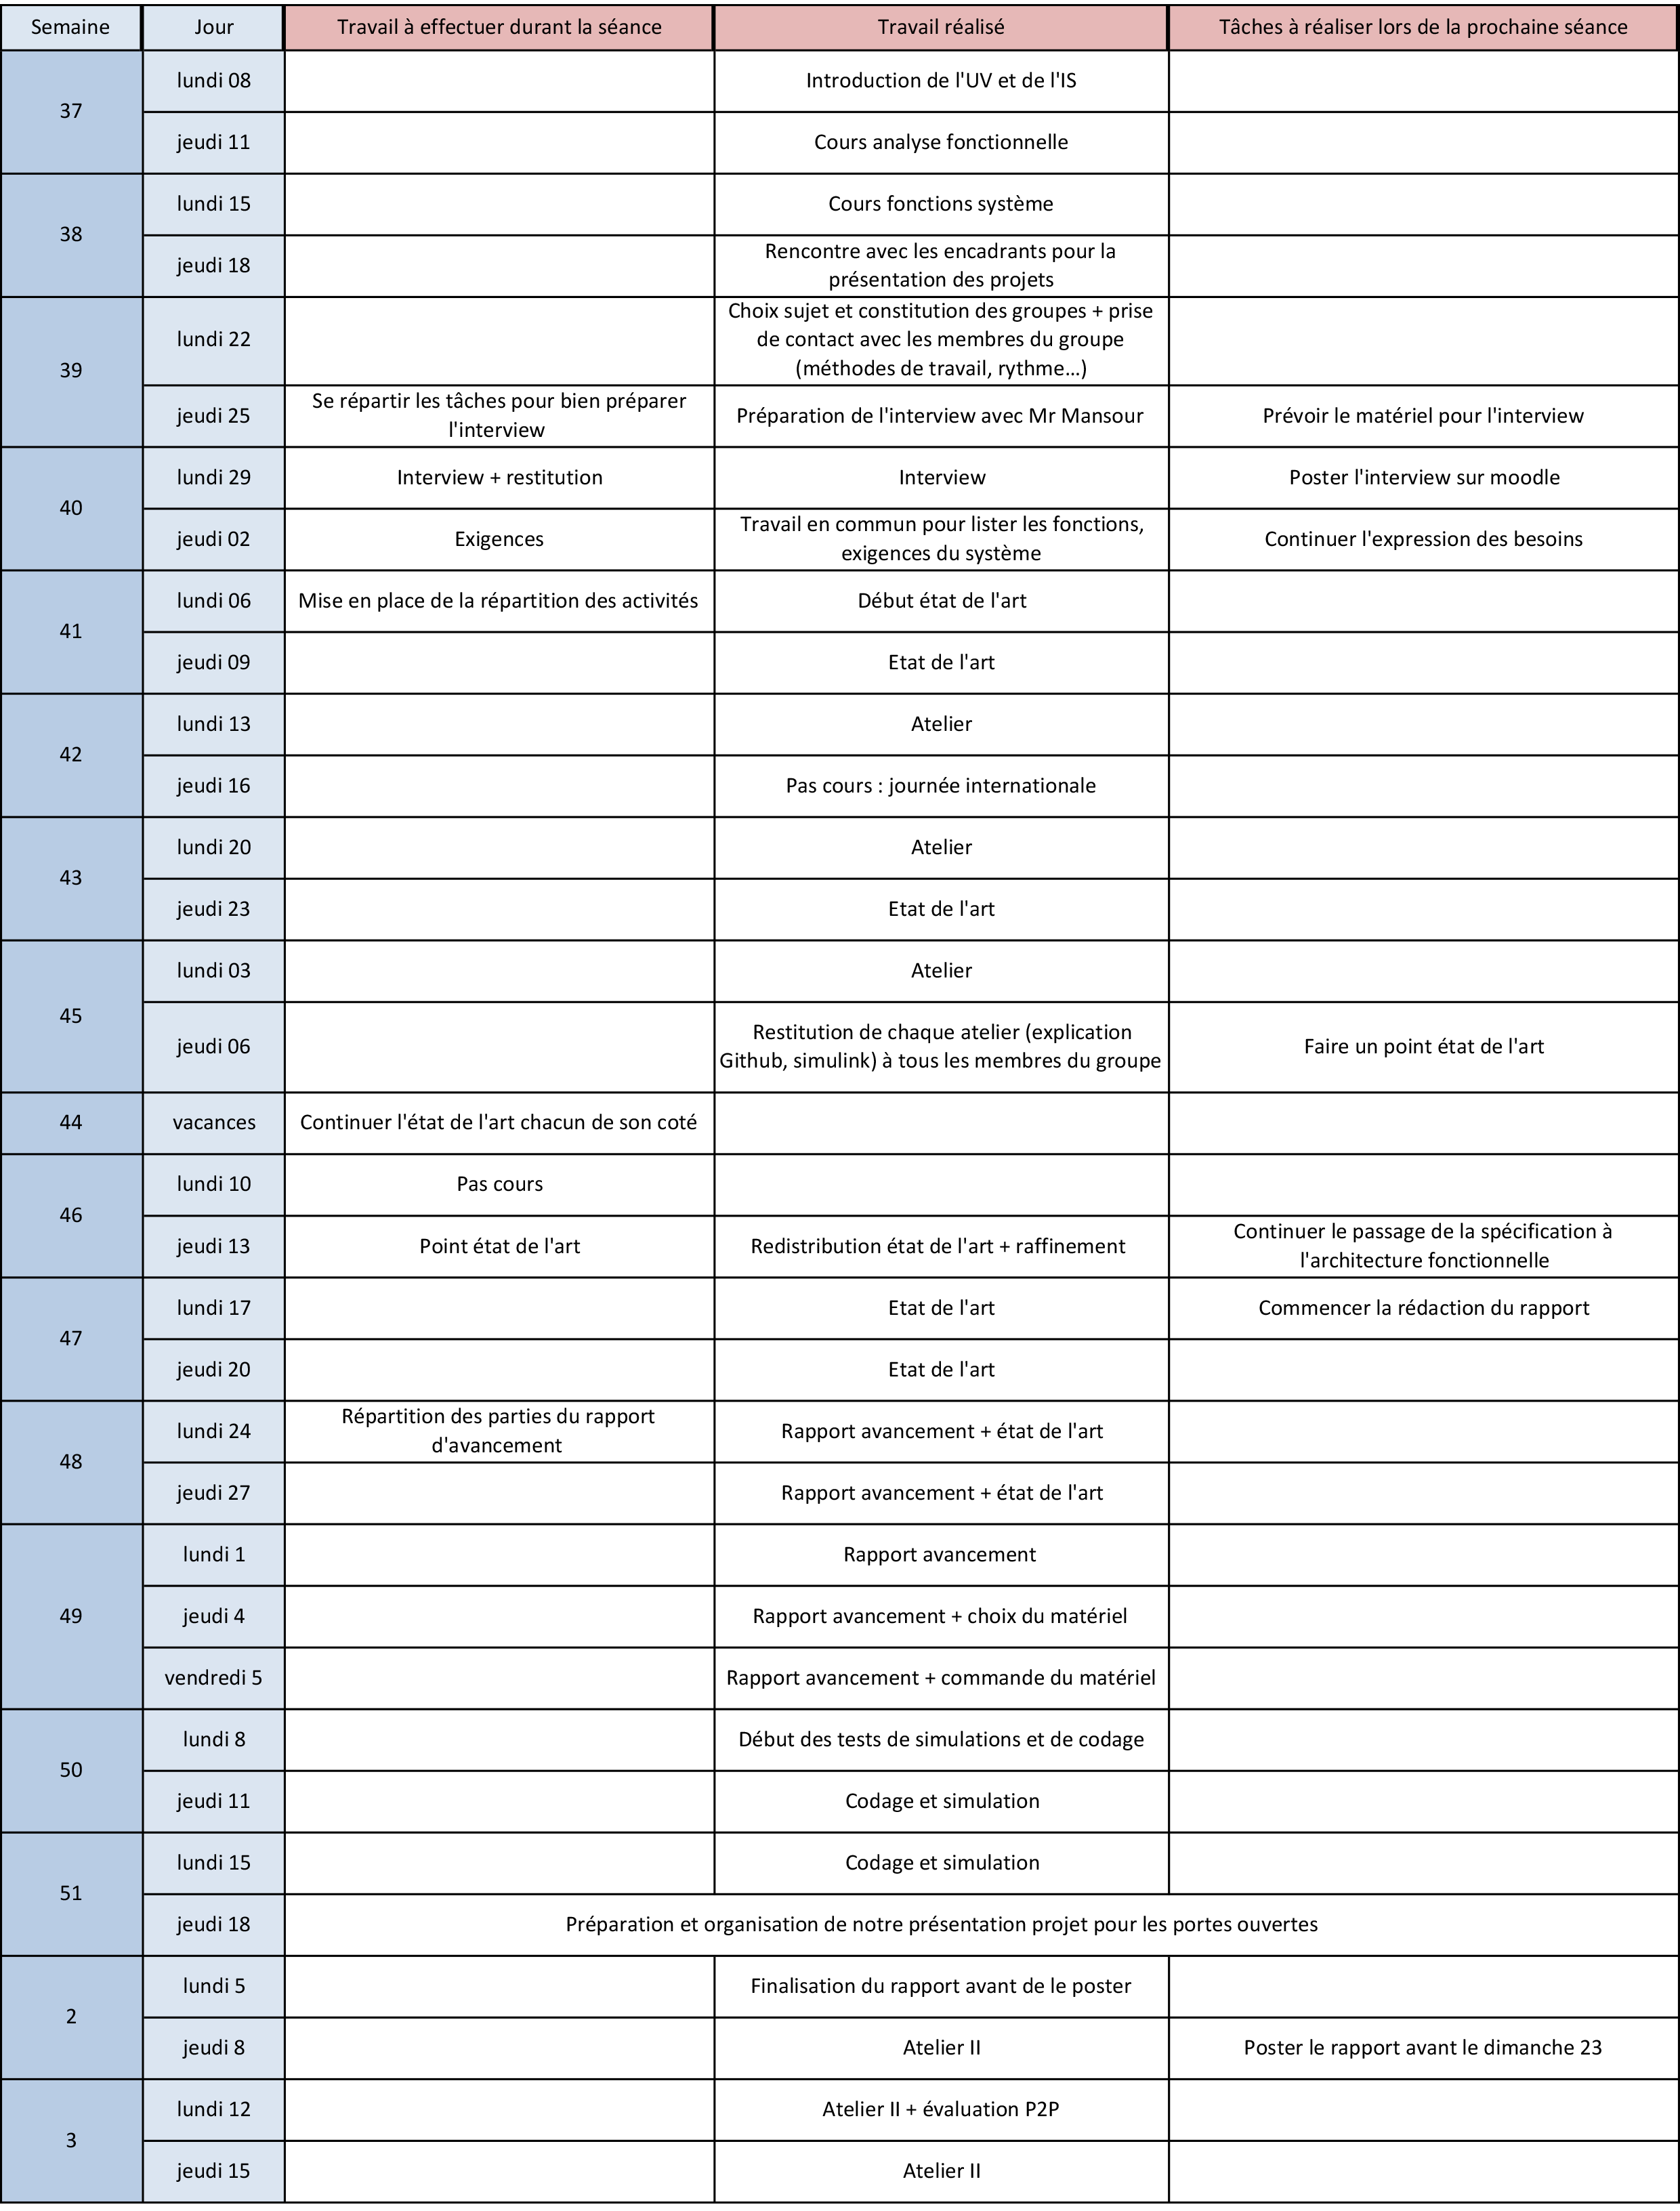
\includegraphics[scale=0.7]{CarnetBord}
  \caption{Carnet de bord}
  \label{fig:CarnetBord}
\end{figure}

Ainsi chacun peut gérer au mieux l'ampleur de la tache à réaliser en fonction du temps qui lui est imparti.
 
Avant chaque séance, nous faisons un point pour fixer les objectifs du jour, de même en fin de séance pour fixer les objectifs de la prochaine séance. 
En milieu de chaque séance, nous nous réunissons pour voir l'avancement de chacun et redéfinir les tâches si nécessaire. 

\begin{figure}[h]
  \centering
  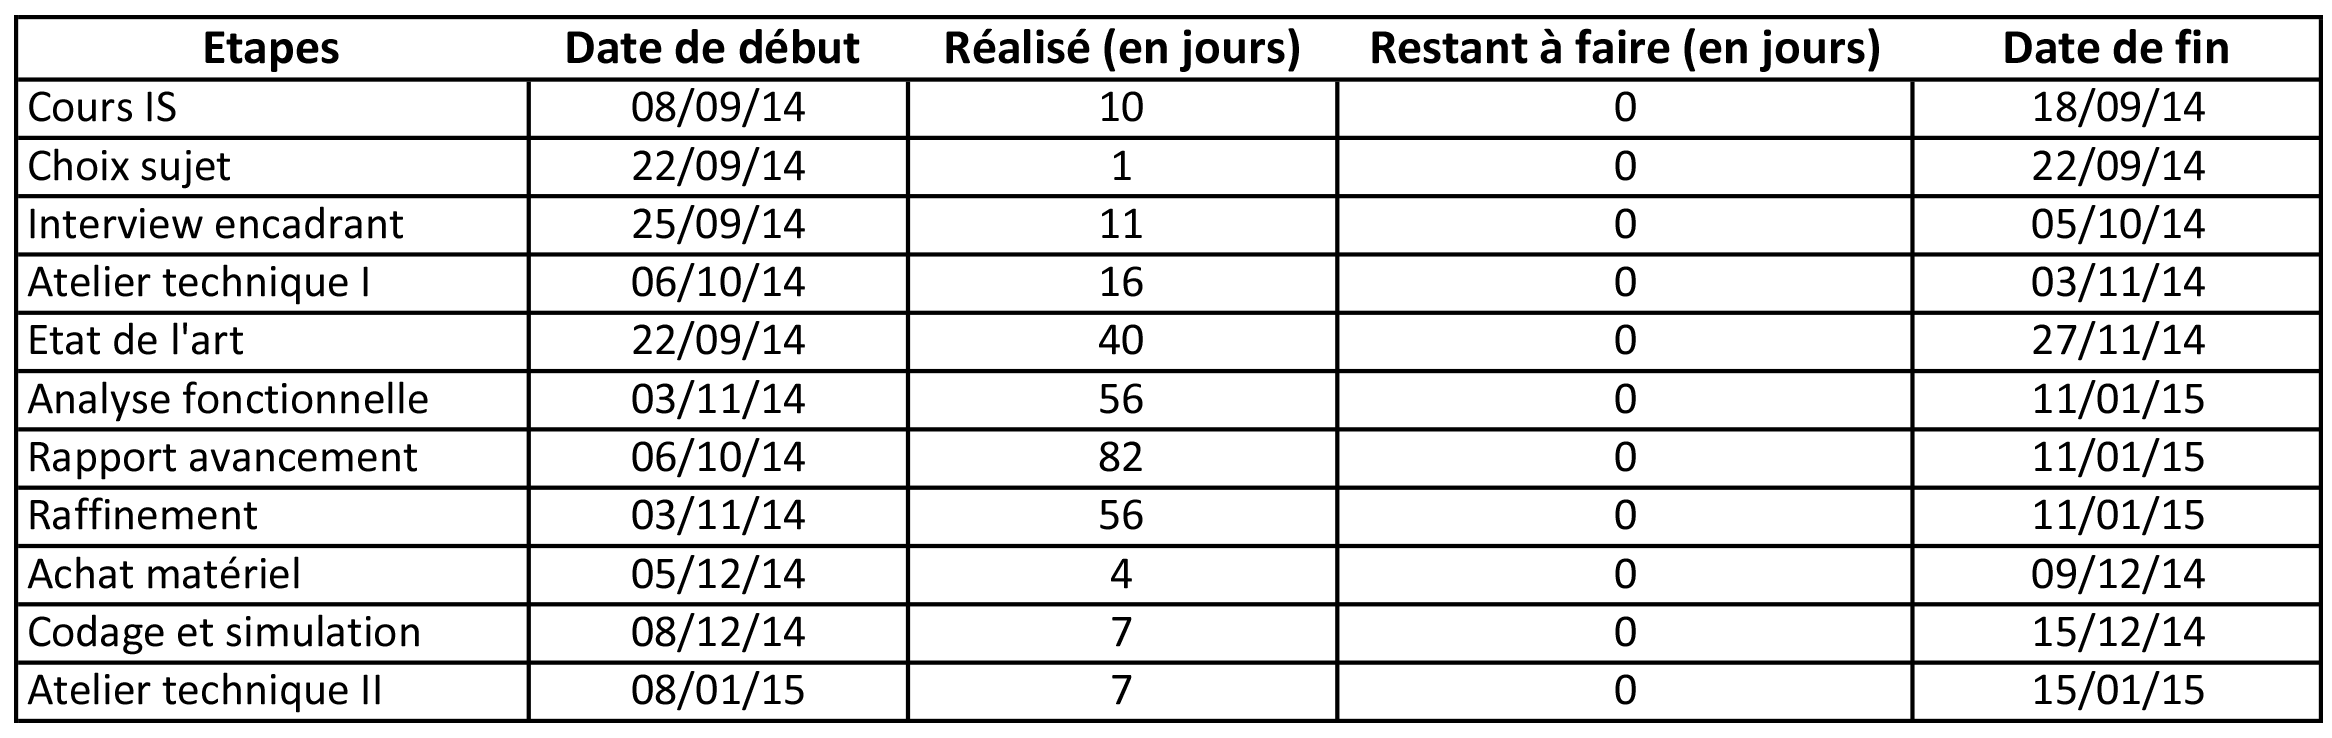
\includegraphics[scale=0.8]{Gantt}
  \caption{Diagramme de Gantt}
  \label{fig:Gantt}
\end{figure}
